\documentclass[11pt, oneside,table]{article}   	% use "amsart" instead of "article" for AMSLaTeX format
%\usepackage{geometry}                		% See geometry.pdf to learn the layout options. There are lots.
\usepackage[margin=.9in]{geometry}
\geometry{letterpaper}                   		% ... or a4paper or a5paper or ... 
%\geometry{landscape}                		% Activate for for rotated page geometry
\usepackage[parfill]{parskip}    		% Activate to begin paragraphs with an empty line rather than an indent
\usepackage{graphicx}				% Use pdf, png, jpg, or eps� with pdflatex; use eps in DVI mode
\usepackage{moreverb}						% TeX will automatically convert eps --> pdf in pdflatex		
\usepackage{amssymb}
\usepackage{mathtools}
\usepackage[framed,numbered,]{mcode}
\usepackage{listings}
\usepackage{xcolor}
\usepackage{amsmath}
\usepackage{placeins}
\usepackage{float}
\restylefloat{table}
\lstset { %
    backgroundcolor=\color{black!7}, % set backgroundcolor
    basicstyle=\footnotesize,% basic font setting
}

\newcommand{\bigo}{$\mathcal{O}$}

\title{MATH 6644\\Project 2}
\author{Stephan Boettcher}
%\date{}                                           % Activate to display a given date or no date

\begin{document}
\maketitle
\section*{Fixed-point and Newton's Method for Nonlinear systems}

{\it Consider the discrete Chandrasekhar H-equation:

$$F_i(\vec{x})=x_i -(1-\frac{c}{2N}\sum\limits^N_{j=1}\frac{\mu_ix_j}{\mu_i+\mu_j})^{-1}=0
$$
where $c \in(0,1)$ is a given constant, $\mu_i=\frac{(i-\frac{1}{2})}{N}$ for $1\le i \le N$ and $N$ is the dimension of the unknown vector $\vec{x}$. Write your own code and compute the solution of the equation for $N=200$ and $c=0.9$ by using:
\begin{enumerate}
\item Fixed-point method,
\item Chord method,
\item Newton method,
\item Shamanskii method with $m=2$.
\end{enumerate}
In all of the computations, the initial guess is taken as $\vec{x}=[1,1,\dots,1]^T$ and the stopping condition is given.
}\\


The Chandrasekhar H-equation was introduced by astrophysicist Subrahmanyan Chandrasekhar is used to solve exit distribution problems in radiative transfer. In the world of Numerical Methods, this equation serves as a well-understood problem that nonlinear solvers can tackle. In this project, the Fixed point and variations on Newton's methods were used to solve the discrete Chandrasekhar H-equation with a constant of $c=0.9$ and $N=200$. These four methods are all able to solve nonlinear systems of equations with various rates of convergence. For all of these methods, the standard assumptions are held.

\subsection*{Fixed-Point Method}
The Fixed point method is a nonlinear solver that relies on contraction mapping to find a solution. The Fixed point iteration is given by:
$$ \vec{x_{n+1}}=\vec{x_n}-F(\vec{x_n})
$$
By inducing a contraction mapping, given by $ \vec{x}=k(\vec{x})$, the method will converge, so long as the following conditions are met:
$$||k(\vec{x})-k(\vec{y})||\le \gamma ||\vec{x}-\vec{y}|| \ \ \ \ 0<\gamma<1
$$
where $k(\vec{x})=\vec{x}_{n+1}$, $k(\vec{y}),\vec{y}=\vec{x}^*$ and $\gamma$ is a constant.  The Fixed-point method may not converge as quickly as other methods, but it is a relatively straight forward method and does not need to calculate a Jacobian matrix to converge. This can be a huge advantage over the Newton's family of methods, should finding the Jacobian prove to be difficult or costly.

\subsection*{Newton Method}
Newton's method is a numerical method that iteratively finds successively better approximations to the zeros of a real function. The Newton iteration is defined as:
$$\vec{x}_{n+1}=\vec{x}_n-\frac{F(\vec{x}_n)}{F'(\vec{x}_n)}
$$
where $F(\vec{x})$ is the value of the function $F$ at $\vec{x}$ and  $F'(\vec{x})$ is the derivative of $F(\vec{x})$. Newton's method has an advantage over the Fixed point method when looking at the convergence rate. While the Fixed point method is expected to converge at a linear rate, Newton's method is able to converge quadratically. The convergence rate is governed by:
$$||\vec{x}_{n+1}-\vec{x}^*||\le k||\vec{x}_n-\vec{x}^*||^2
$$
where $\vec{x}^*$ is the solution and k is a constant governed by $0<k<1$. As can be seen by the squared term on the right hand side, the error should be decreasing at a quadratic rate. One issue with Newton's method is solving the step $F'(\vec{x}_n)\vec{s}=-F(\vec{x}_n)$. This step requires not only solving a linear system of equations, but also requires the formation of the Jacobian at each step. If the Jacobian is costly to evaluate, this method may take more time to converge, while still having fewer iterations, than other methods. 


\subsection*{Chord Method}
The Chord method is a variation on Newton's method that attempts to minimize the cost of evaluating the Jacobian. The  iterative step used in the Chord method is nearly identical to that of Newton's method, but has one small change:
$$\vec{x}_{n+1}=\vec{x}_n-\frac{F(\vec{x}_n)}{F'(\vec{x}_0)}
$$
Instead of using a Jacobian calculated at each step, the Jacobian is calculated at the start and the LU factorized version of this initial Jacobian is used for the rest of the iterations:
$$LU\vec{s}=-F(\vec{x}_n)
$$
By only having to calculate the Jacobian once and only factoring it once, the Chord method is able to speed up the computation at the cost of more iterations. The Chord method gives up the quadratic convergence of Newton's method to achieve speedups in computation. The error of the Chord method is governed by:
$$||\vec{x}_{n+1}-\vec{x}^*||\le k||\vec{e}_0||\ ||\vec{e}_n||
$$
where $||\vec{e}_0||$ is the norm of the initial error, given by $||\vec{e}_0||=||\vec{x}_0-\vec{x}^*||$, and $||\vec{e}_n||$ is the norm of the error at step n. From the above equation we know that the error converges at a locally linear rate.

\subsection*{Shamanskii Method with $m=2$}
The Shamanskii method attempts to hybridize the Chord method with Newton's method. The Shamanskii method uses the parameter $m$ to determine how many chord iterations will be performed prior to recomputing and refactorizing the Jacobian. This allows the Shamanskii method to maintain a higher order convergence while still minimizing the number of times the Jacobian is computed. If $m=1$, the Shamanskii method becomes Newton's method and converges at the same rate. The error of the Shamanskii method is governed by:
$$||\vec{e}_{n+1}||\le k_s||\vec{e}_n||^{m+1}
$$
where $||\vec{e}_n||=||\vec{x}_n-\vec{x}^*||$, and $k_s$ is a constant. From the above equation, we know that the Shamanskii method will converge at a higher order rate, assuming the standard assumptions hold.

\subsection*{Results}

The four numerical methods described above were used to solve the discrete Chandrasekhar H-equation given by:
$$F_i(\vec{x})=x_i -(1-\frac{c}{2N}\sum\limits^N_{j=1}\frac{\mu_ix_j}{\mu_i+\mu_j})^{-1}=0
$$
where $c \in(0,1)$ is a given constant, $\mu_i=\frac{(i-\frac{1}{2})}{N}$ for $1\le i \le N$ and $N$ is the dimension of the unknown vector $\vec{x}$. Initially, the $\vec{x}_0$ was set to $[1,1,\dots,1]^T$.  To determine the most effective solver for this problem, the following two metrics were considered:
\begin{enumerate}
\item Number of iterations required to converge
\item Time to converge (Cost of the method)
\end{enumerate}
 
Once all four methods were run, the relative error at each iteration was plotted, as seen in Figure \ref{c}, to graphically illustrate the convergence rate. The Fixed point and Chord methods can be seen to have linear convergence rates and require far more iterations to converge than the Newton or Shamanskii methods. The Newton and Shamanskii methods both seem to converge at a quadratic rate, with the Shamanskii method having a slightly slower rate. The rate of convergence for the Shamanskii method was somewhat surprising as it was expected to converge at a cubic rate. Instead, this method converged slightly slower than the quadratic Newton's method. Regardless, both the Shamanskii and Newton's method were able to converge in 8 iterations.
 
 While both metrics are important to consider when evaluating a numerical method, the runtime of the method is generally considered more important.  Figure \ref{tab} gives not only the number of iterations required to converge, but the runtime of each method. The Final Error column shows the final error of each method. The stopping condition, given in the problem statement, evaluates to $\approx 1.453*10^{-6}$. Once a method's relative error is below this point, it is able to stop executing.
 
 While the Shamanskii and Newton's methods both converge in the fewest number of iterations, Newton's method actually takes $\approx$ 100 times longer to run than the Fixed Point method. Creating and evaluating the Jacobian is a costly step for this equation. It takes the \mcode{diffjac} code $\approx 0.375s$ to evaluate, thus contributing the most to the runtimes of the codes. Since the Fixed Point method does not rely on the Jacobian for its convergence, it is able to run significantly faster. The Chord method is the second fastest method as it only requires evaluating the Jacobian once. Comparing the cost of evaluating the Jacobian to the runtime of the Chord method reveals that the Jacobian is the primary driver of the runtime. Once evaluated, the chord method was able to run with approximately the same speed as the Fixed Point method. 
 
 \begin{figure}[htbp]
\begin{center}
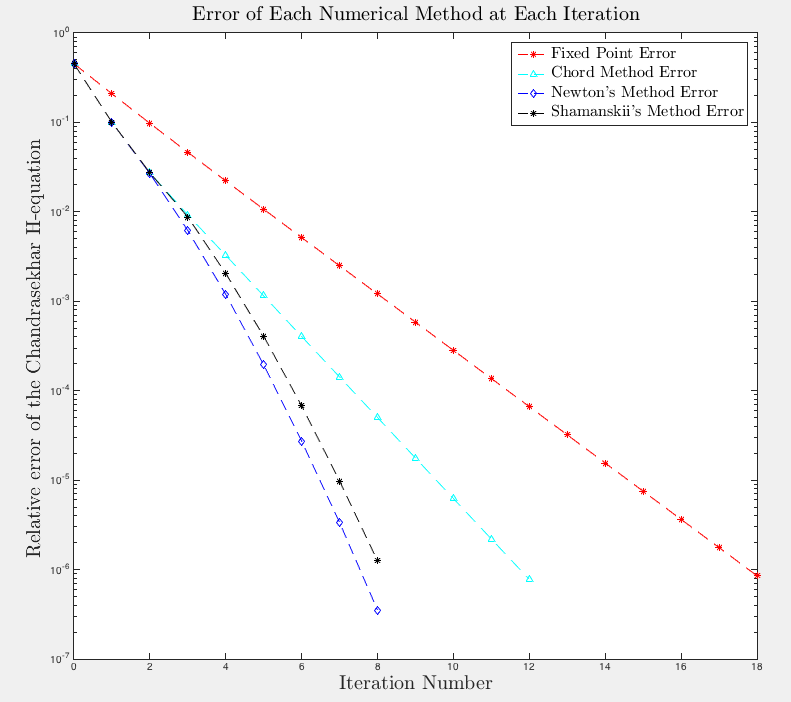
\includegraphics[width=120mm]{converge.png}
\caption{The error of each method at a given iteration}
\label{c}
\end{center}
\end{figure}
 \FloatBarrier

\begin{figure}[htbp]
\begin{center}
\begin{tabular}{ | c|c|c| c|}
\hline
Numerical Method  &Iterations Required to Converge & Time to Converge & Final Error \\\hline
Fixed Point&18& 0.037566& $8.526859*10^{-7}$\\\hline 
Chord&12& 0.401574& $7.749982*10^{-7}$\\\hline 
Shamanskii's Method&8& 1.51895776& $1.248676*10^{-6}$\\\hline 
Newton's Method&8& 3.03898413&$ 3.506771*10^{-7}$\\\hline

  % Design2 &300 & 380 & 370 & 34 & 40& 400& 100& 50& 100& 100 \\\hline
%  Design3 &300 & 600 & 580 & 40 & 50& 550& 100& 150& 200& 250 \\\hline

\end{tabular}
\caption{Final Results of the 4 methods }
\label{tab}
\end{center}
\end{figure}



\subsection*{Conclusions}
  

%\begin{figure}[htbp]
%\begin{center}
%\begin{tabular}{ | l | c|c| c| c | c | c| c| c| c  | c | }
%\hline
%  &A & B & C &D &E&F&G&H&I&J\ \\\hline
%  Design1 &240 & 350 & 305 & 30 & 35& 400& 90& 0& 30& 300 \\\hline
%% Design2 &300 & 380 & 370 & 34 & 40& 400& 100& 50& 100& 100 \\\hline
%%  Design3 &300 & 600 & 580 & 40 & 50& 550& 100& 150& 200& 250 \\\hline
%
%\end{tabular}
%\caption{Design 1 Parameters}
%\end{center}
%\end{figure}
%
%The isometric view of this design can be seen in Figure \ref{d1i}. The large cylinder was plotted using multiple instances of the \mcode{surf} command on two cylinders. Figure \ref{d1y} and Figure \ref{d1z} show the printer design in the X-Y and X-Z plains, respectively.
%
%\begin{figure}[htbp]
%\begin{center}
%\includegraphics[width=160mm]{d1iso.png}
%\caption{An isometric view of Design 1}
%\label{d1i}
%\end{center}
%\end{figure}



\end{document}  